\documentclass[12pt,a4paper,UTF8]{article}
% \usepackage{ctex} % Chinese support
\usepackage{graphicx} % Insert images
\usepackage{listings} % Print source code
\usepackage{color} % Color support
\usepackage{booktabs} % Professional table support
\usepackage{pdflscape} % Landscape pages support in PDF
\usepackage{hyperref} % Hypertext links support for cross-referencing

% Customize hyperref format (it's set to no special format here)
\hypersetup{hidelinks}

% Declare directories to search for graphics files for graphicx
\graphicspath{{figures/}{logo/}}

% Define source code style for listings
\lstdefinestyle{python}{
  language=Python,
  basicstyle=\ttfamily\footnotesize,
  keywordstyle=\bfseries\color[rgb]{0, 0, 1},
  identifierstyle=\color[rgb]{0.5, 0.3, 0.1},
  stringstyle=\color[rgb]{0.6, 0.1, 0.1},
  commentstyle=\itshape\color[rgb]{0.05, 0.5, 0.05},
  backgroundcolor=\color[gray]{0.95},
  numbers=left,
  numbersep=5pt,
  numberstyle=\color[gray]{0.6},
  breaklines=true
}

% Define new command for title page
\newcommand{\reporttitle}[2]{
  \LARGE\textsf{#1}\quad\underline{\makebox[12em]{#2}}
}
\newcommand{\reportinfo}[2]{
  \large\makebox[4em]{\textsf{#1}}\quad\underline{\makebox[18em]{#2}}
}

% The document begins here
\begin{document}
\begin{titlepage}
  \centering
  \vspace*{\fill}
  
\includegraphics[height=144pt]{nju-logo}\\[48pt]
  {\huge\textsf{Lab Report}}\\[48pt]
  \reporttitle{Lab Name}{Arp}\\[72pt]

  \reportinfo{Course}{Computer Network}\\[8pt]
  \reportinfo{Major}{Computer Science and Technology}\\[8pt]
  \reportinfo{Id}{191220129}\\[8pt]
  \reportinfo{Name}{Shangyu.Xing}\\[8pt]
  \reportinfo{Email}{191220129@smail.nju.edu.cn}\\[8pt]
  \reportinfo{Date}{2021.04}\\
  \vspace*{\fill}
\end{titlepage}

\tableofcontents
\newpage

\section{Objective}
\begin{itemize}
	\item Learn address resolution protocol and how to implement it;
	\item learn to implement hardware logic using the Switchyard framework;
	\item learn to capture network package using wireshark.
\end{itemize}

\section{Requirements}
This lab requires to implement a router who can respond to ARP requests and cache an ARP table.
\begin{itemize}
	\item Handle ARP request;
	\item implement a cached ARP table.
\end{itemize}

\section{Procedure}
In this section, I will explain how I implement the router in detail. \\

\subsection{Handle ARP Request}
The logic to handle ARP request is very simple. The procedure is listed as follows:
\begin{enumerate}
	\item Upon receiving a packet, get its header to check whether it is an arp packet;
	\item if it is, check all the router's interfaces. If there is a match, create the arp reply packet and send it out through the same interface which the arp request come in; else do nothing.
\end{enumerate}
\lstinputlisting[style=python]{1.py}

\subsection{Cached ARP Table}
To maintain an arp table, we should create a python class for it. The class consists of a constant indicating timeout value and a dict which stores (ip -> (mac, timestamp)) as an entry of table. It has the following methods:
\begin{itemize}
	\item update -- create an entry or update the timestamp of a specific entry;
	\item get -- query for mac address with an ip;
	\item \_str\_ -- its representation in str when printing.
\end{itemize}
\lstinputlisting[style=python]{2.py}
Note that when an entry timeout, it is not physically deleted; instead it is marked invalid when querying or printing. \\
To update the table and print it out when an arp packet arrives, we should add the following lines at the end of function 'handle\_packet':
\lstinputlisting[style=python]{3.py}

\section{Result}
\subsection{Handle ARP Request}
Firstly I tested my code with switchyard testcases:
\begin{figure}[htbp]
	\centering
	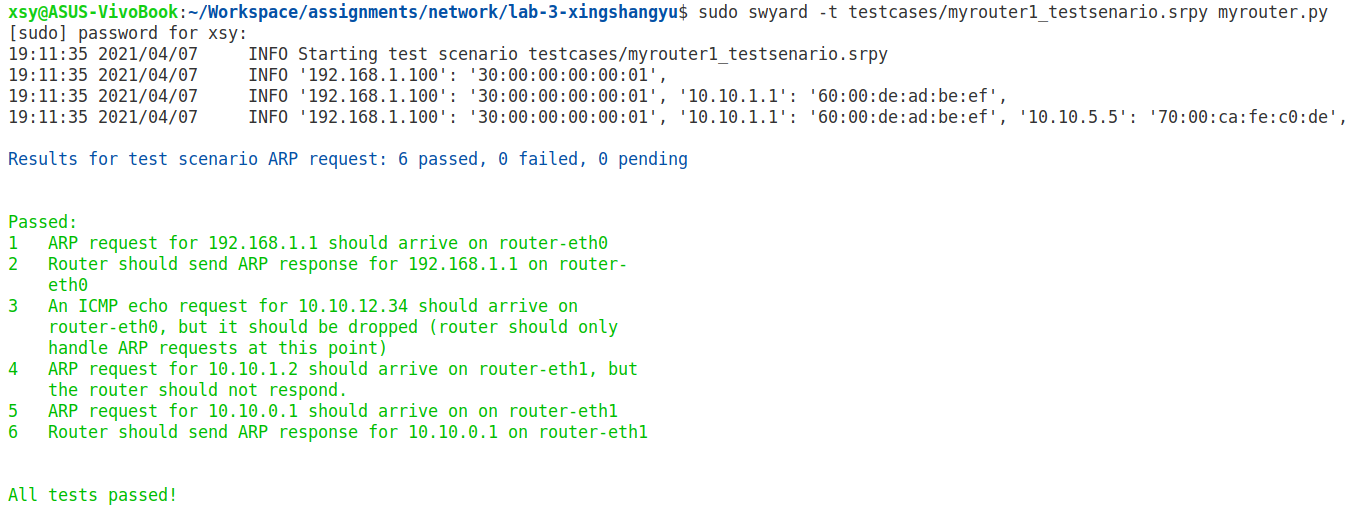
\includegraphics[width=\textwidth]{4}
	\caption{Switchyard test result}
\end{figure}
\\
To perform a test in mininet, I commanded server1 to ping the router 3 times and ran wireshark on server1. I got a result of 100\% drop and this record:
\begin{figure}[htbp]
	\centering
	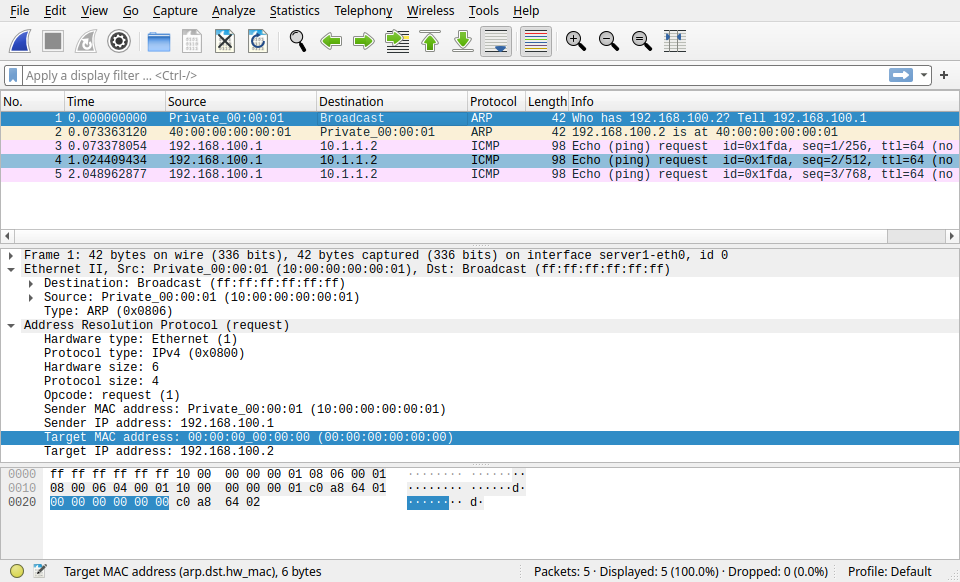
\includegraphics[width=\textwidth]{1}
	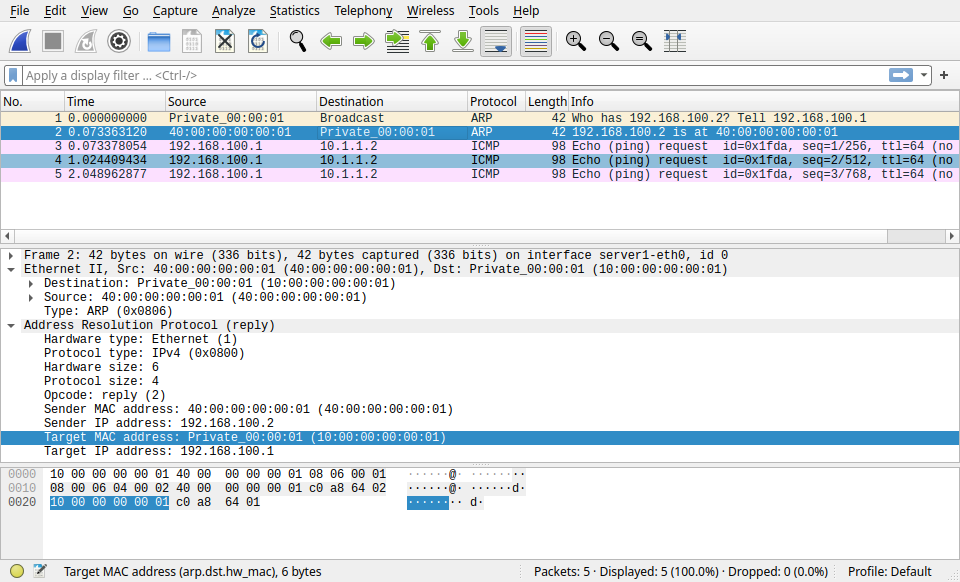
\includegraphics[width=\textwidth]{2}
	\caption{Wireshark capture result}
\end{figure}
\newpage
What happened in the network was this:
\begin{enumerate}
	\item Server1 broadcast arp packet, and the router found that it was directed at it;
	\item The router made an arp response to server1;
	\item Server1 extract mac from the response, then sent echo requests packet to the router three times subsequently;
	\item the router received echo requests, but didn't reply.
\end{enumerate}
As a result, wireshark could capture arp request/response and echo request but no echo response.

\subsection{Cached ARP Table}
I set the timeout value to 10 second, and made the following commands:
\lstinputlisting[style=python]{4.py}
Router's log (which contains the cached table at different timestamp):
\begin{figure}[htbp]
	\centering
	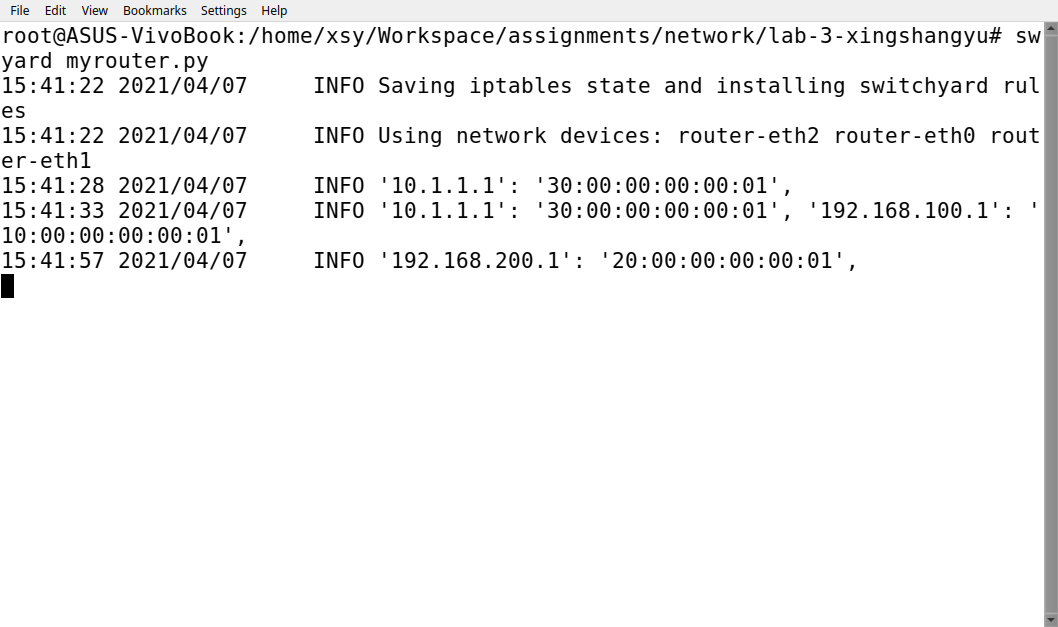
\includegraphics[width=\textwidth]{3}
	\caption{Router's log in mininet}
\end{figure}
\newpage
As can be seen in the picture above, the entries in the arp table did not timeout in 5s but timeout after 15s. The detailed procedure is this:
\begin{enumerate}
	\item Client broadcast arp packet, and the router stored client's (ip -> (mac, timestamp)) in its arp table;
	\item The router made an arp response to client;
	\item Client sent echo requests packet to the router, but it didn't reply;
	\item Server1 did the same thing, and the router stored server1's (ip -> (mac, timestamp)). At this time, the previous entry (which is the client's information) had not timeout, so the table now contained 2 entries;
	\item Server2 did the same thing, and the router stored server2's (ip -> (mac, timestamp)). At this time, the previous entries (which are the client's and server1's information) had timeout, so the table now contained 1 entry.
\end{enumerate}

\section{Summary}
\begin{itemize}
	\item Knowing how to use tools effectively will greatly enhance working efficiency;
	\item English reading and writing skills are important.
\end{itemize}

\end{document}